\section{Einleitung}
%%%%%%%%%%%%%%%%%%%%%%%%%%%%%%%%%%%%%%%%%%%%%%%%%%%%%%%%%%%%%

 Das Nervensystem ist das wohl komplizierteste System des menschlichen Körpers. Die Funktionsweise dieses komplexen Kommunikationssystems ist bis heute nicht gänzlich erforscht. Jedoch können durch andauernde Forschung immer mehr Kenntnisse gewonnen werden. Die funktionelle Untereinheit des Nervensystems ist die Nervenzelle. Diese Nervenzellen oder Neurone sind in der Lage Informationen elektrisch oder chemisch an andere Nervenzellen oder nachfolgende Strukturen zu übertragen. Das Nervensystem des Menschen ist aus 86.1 \rpm 8.1 Millionen Nervenzellen aufgebaut \textsuperscript{\cite{azevedo2009equal}}, die ein verzweigtes Netzwerk bilden \textsuperscript{\cite[Kap.~1]{trepel2011neuroanatomie}}. Die Großhirnrinde des menschlichen Gehirns, als Teil des Nervensystems, kann aufgrund lokaler, histologischer Charakteristika, wie beispielsweise unterschiedliche Schichtung verschiedener Neuronen-Typen, in 52 voneinander abgrenzbare Areale, die sogenannten \textbf{Brodmann-Areale}\index{Brodmann-Areale}, unterteilt werden (Abb.~\ref{fig:brodmann_areale}). Obwohl diese Areale bereits Anfang des zwanzigsten Jahrhunderts definiert wurden, dienen sie bis heute zur Beschreibung distinkter Hirnareale. So ist das Brodmann-Areal 17 heute mit der primären Sehrinde, das Areal 41 mit der primären Hörrinde gleichzusetzen. Das Brodmann-Areal 6, sowie Teile des Areals 8, beschreiben den prämotorischen Cortex \textsuperscript{\cite[Kap.~9]{trepel2011neuroanatomie}}. Die Beständigkeit der von Brodmann festgelegten Areale dienen als Beispiel des Zusammenspiels von Morphologie und Funktion funktioneller Systeme. Sie zeigen, dass die Struktur des Systems die Grundlage der zugehörigen Funktion ist.

\begin{figure}[H]
    \centering
    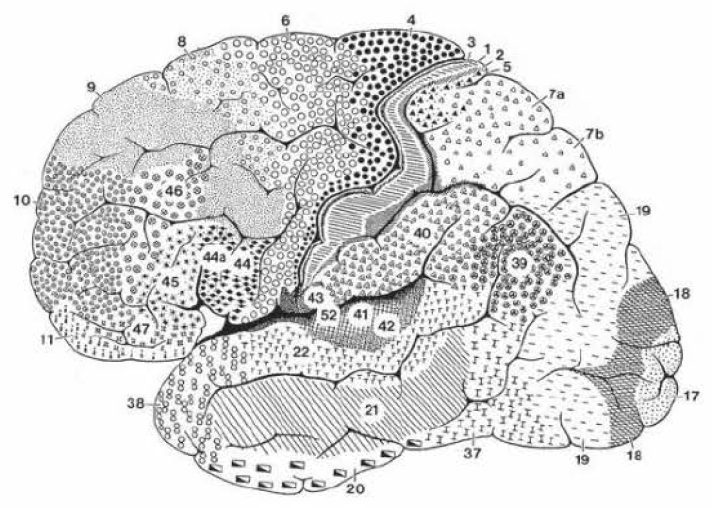
\includegraphics[width=0.7\textwidth]{pictures/Bilder_Jule/Andere/brodmann.PNG}
    \caption[Brodmann-Areale]{\textbf{Brodmann-Areale.} Die Großhirnrinde wurde durch Brodmann aufgrund histologischer Merkmale in 52 Areale unterteilt. \\
    Abbildung aus \textit{Neuroanatomie}, Trepel \textsuperscript{\cite[Kap.~9]{trepel2011neuroanatomie}}.}
    \label{fig:brodmann_areale}
\end{figure}

Um die zugrundeliegende Struktur des Nervensystems, bzw. des Gehirns, besser beschreiben zu können, werden unterschiedliche Ebenen herangezogen (Abb.~\ref{fig:schnittebenen}). Die rostro-caudale Achse beschreibt die Achse zwischen Kopf (rostral) und Schwanz (caudal) eines Tieres, die dorso-ventrale Achse die zwischen Rücken (dorsal, posterior) und Bauch (ventral, anterior). In Bezug auf das Gehirn kann, vor allem beim Menschen, noch zwischen oben (superior) und unten (inferior) unterschieden werden. Des Weiteren existieren drei verschiedene (Schnitt-)Ebenen: die Horizontal-, Sagittal- und Coronal-Ebene \textsuperscript{\cite[Kap.~15]{kandel2013principles}}. Ziel dieses Protokolls ist es, einen groben Überblick über die grundlegende funktionelle Anatomie des Gehirns zu geben. Es soll ein Verständnis der räumlichen Lage der unterschiedlichen Areale und funktionellen Systeme entstehen. Die wichtigsten funktionellen Untereinheiten, sowie die sensorischen und motorischen Bahnen, die integrativen Systeme und die generellen Transmittersysteme sollen genauer beschrieben werden.

\begin{figure}[H]
    \centering
    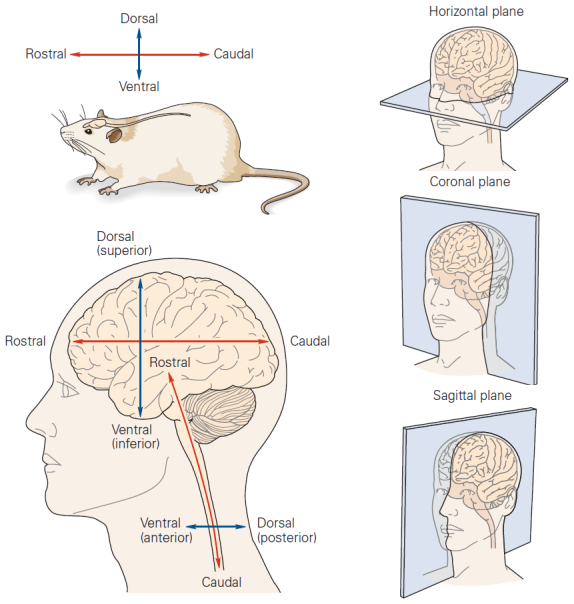
\includegraphics[width=0.7\textwidth]{pictures/Bilder_Jule/Andere/Schnittebenen.png}
    \caption[Achsen und Schnittebenen]{\textbf{Achsen und Schnittebenen.}\\
    Abbildung aus \textit{Principles  of Neural Science}, Kandel et al. \textsuperscript{\cite[Kap.~15]{kandel2013principles}}.}
    \label{fig:schnittebenen}
\end{figure}{}